\documentclass[english,11pt,twoside,a4paper]{article}
\usepackage[left=2cm,top=1cm,right=2cm,nohead,nofoot]{geometry}
\usepackage[utf8]{inputenc}
\usepackage{hyperref}
\usepackage{amssymb}
\usepackage{graphicx}
\begin{document}
\author{
  Niemistö, Jesse
  \and
  Muona, Leo
  \and
  Hilden, Matias
}
\title{Requirements and design}

\maketitle

\section{Introduction}
This document includes requirements, features and design of our turret for Intelligent Embedded Systems -course (University of Helsinki course number 582711). For our project we chose to create an "intelligent" turret inspired by video game Portal by Valve Company. This document describes the intended features that our turret will have. This includes different subsections of the project, including audio output, camera input, DC motor control system and software.

\section{Features}
TODO
- fancy use case picture?

\section{Audio}

For audio we will be using the 3.5mm jack audio output connector on the raspberry pi. However, instead of connecting just some ready stereo system, we'll build our own audio amplifier, which is connected to a single speaker. Thus we'll only need to output mono audio. Since audio will mostly contain speaking, it does not matter. The used speaker will be small and low powered.

To be able to use our audio amplifier on the raspberry pi, we need to make a simple connector, which is quite simple. We only need to get a male 3.5mm jack connector, ignore the possible second audio output (incase of stereo), and solder our two needed wires on it (ground and audio out).

\begin{figure}
  \begin{center}
    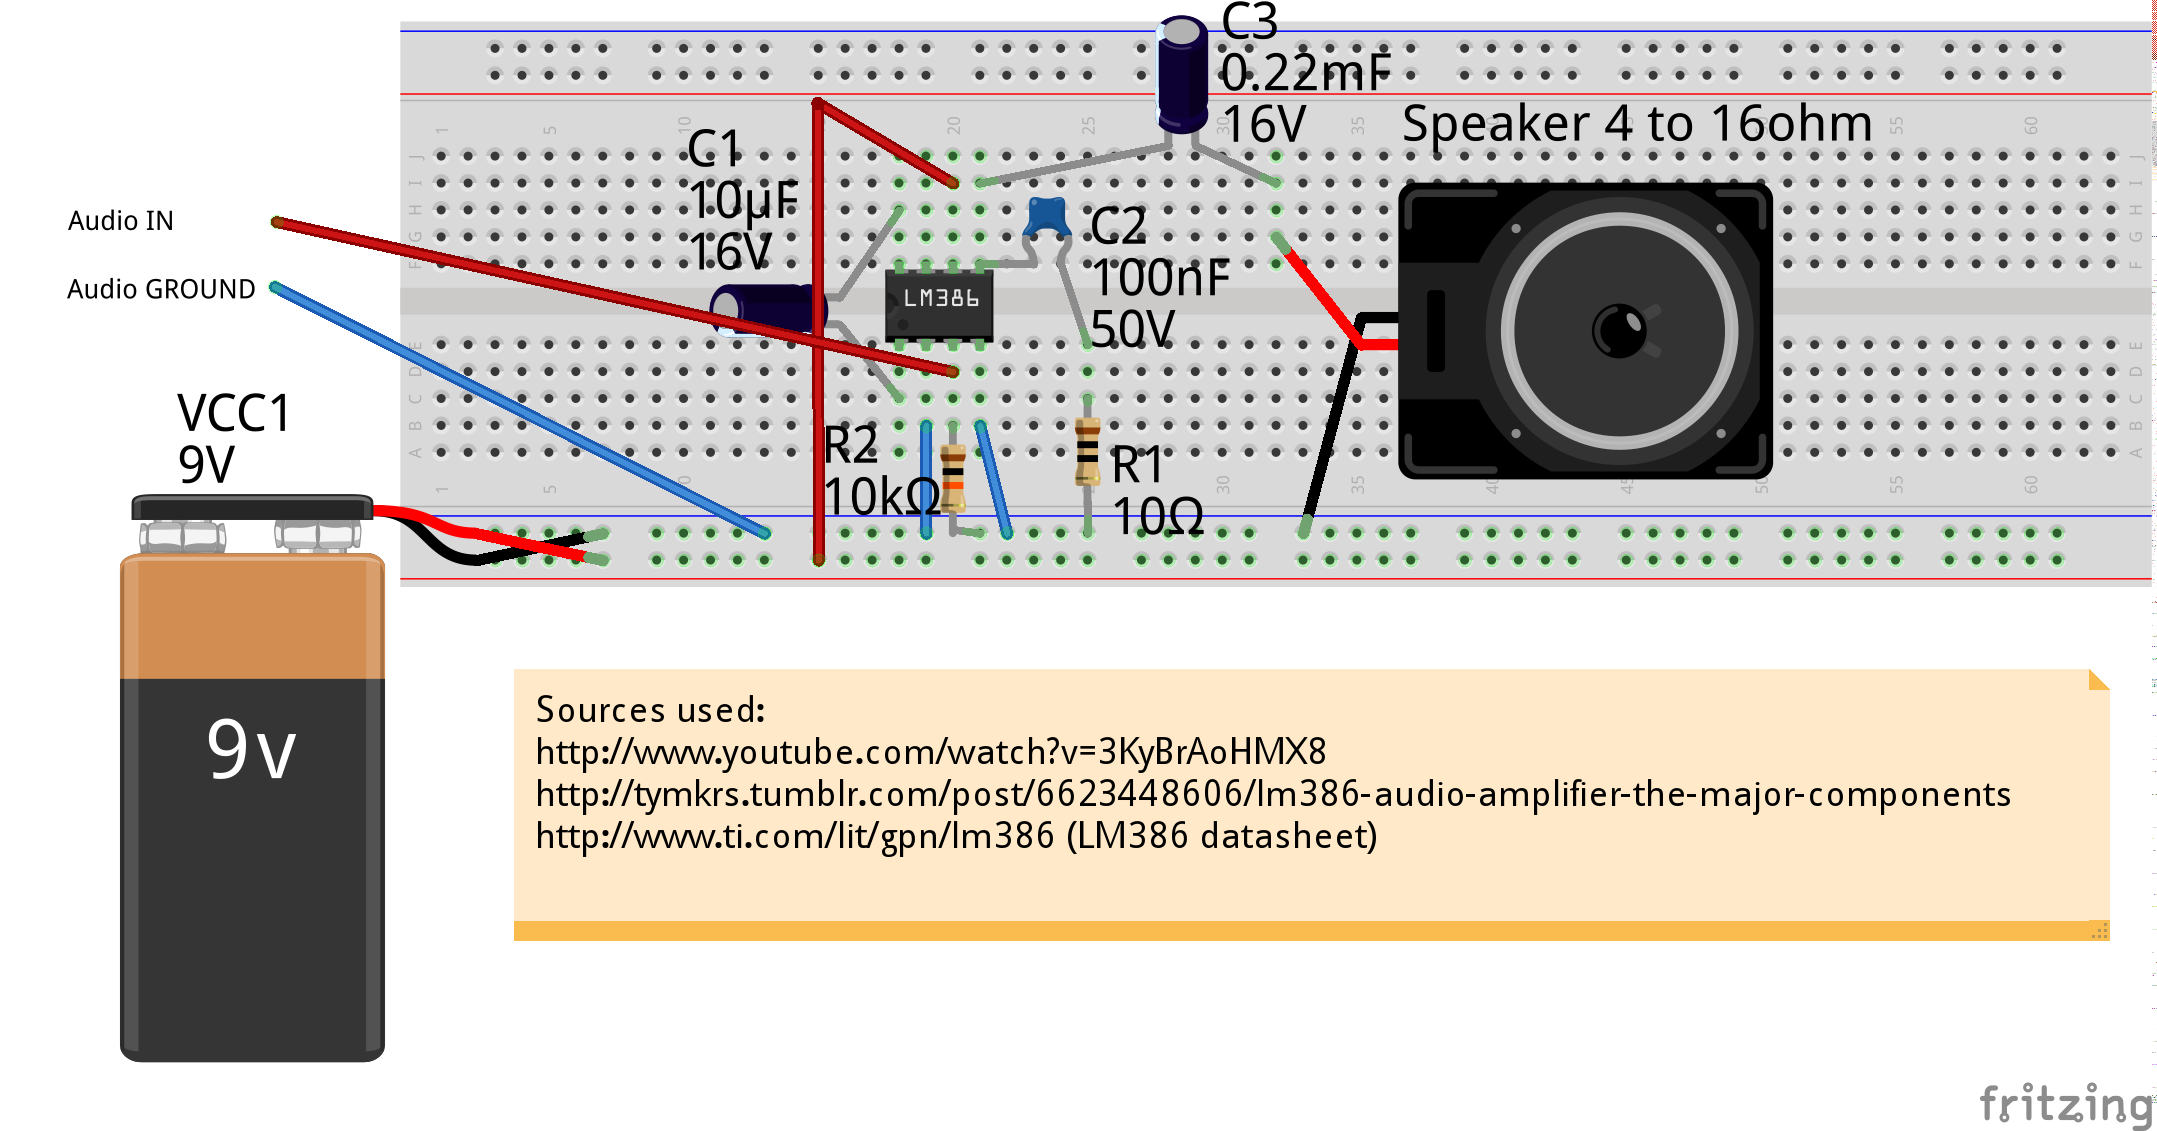
\includegraphics[scale=0.75]{audio_amplifier_lm386_bb.png}
    \caption{Breadboard view for the audio amplifier.}
  \end{center}
  \label{lm386_bb}
\end{figure}

In the heart of the audio amplifier stands the LM386 circuit, which is a "Low Voltage Audio Power Amplifier" and is more than enough for our use case. The figure in \ref{lm386_bb} shows the breadboard view that we'll be using for the audio amplifier. The build is same to that what is shown on the LM386 datasheet, "amplifier with Gain = 200". 

\begin{itemize}
  \item Between PINs 1 and 8 is a 10uF capacitor, which causes a gain on 200. In desibels this is around 20. 
  \item PIN 2 is places to ground.
  \item PIN 3 takes the audio input, and is connected to ground through 10k ohm resistor.
  \item PIN 4 is placed to ground.
  \item PIN 5 is the amplified audio output.
  \item PIN 6 takes power
  \item PIN 7 is bybassed, doesn't take connection.
\end{itemize}

\section{Camera}
TODO

\section{Motors}
TODO

\section{Software}
TODO

\section{Testing}
TODO: Maybe include these in the subsections of audio, camera and motors?

\end{document}
